\documentclass[11pt]{beamer}
% 
\usepackage[czech]{babel}
\usepackage[utf8]{inputenc}
\usepackage[IL2]{fontenc}
\usepackage{amsmath, amsthm}
\usepackage{mathtools, mathdots}
\usepackage{color}
\usepackage{graphicx}
\usepackage{wrapfig}
\usepackage{pgffor}

%\usepackage{amsmath, amsthm, amssymb, units, dsfont}
\usepackage{sidecap}
\usepackage{enumerate}
\usepackage{xcolor}

\usepackage{mathtools, mathdots}
\usepackage{pgffor}
\usepackage{pdflscape}
\usepackage{afterpage}
\usepackage{chngcntr}
\usepackage{multirow}
\usepackage{tabulary}

\usepackage{listings}
\usepackage{color}

\usepackage{algorithm}
\usepackage{algorithmic}

\usepackage{breqn}
\usepackage{hyperref}

\usepackage{pgfkeys}

\usepackage{changepage}

\definecolor{darkgreen}{rgb}{0,0.6,0}
\definecolor{darkred}{rgb}{0.6,0,0}
\definecolor{darkblue}{rgb}{0,0,0.6}
\definecolor{darkgrey}{rgb}{0.3,0.3,0.3}
\definecolor{grey}{rgb}{0.6,0.6,0.6} %comment
\definecolor{lightgrey}{rgb}{0.92,0.92,0.92}
\definecolor{terminal}{rgb}{0.9,0.9,0.6}
\definecolor{cmd}{rgb}{0.8,0.8,0.98}
\lstset{ 
        basicstyle=\ttfamily,
%         language=Matlab,                                % choose the language of the code
%       basicstyle=10pt,                                % the size of the fonts that are used for the code
%         numbers=left,                                   % where to put the line-numbers
        keywordstyle=\color{darkblue},
        commentstyle=\color{darkgreen},
        stringstyle=\color{darkred},
%         numberstyle=\footnotesize,                      % the size of the fonts that are used for the line-numbers
        stepnumber=1,                                           % the step between two line-numbers. If it's 1 each line will be numbered
        numbersep=5pt,                                  % how far the line-numbers are from the code
%       backgroundcolor=\color{white},          % choose the background color. You must add \usepackage{color}
        showspaces=false,                               % show spaces adding particular underscores
        showstringspaces=false,                         % underline spaces within strings
        showtabs=false,                                         % show tabs within strings adding particular underscores
%       frame=single,                                           % adds a frame around the code
%       tabsize=2,                                              % sets default tabsize to 2 spaces
%       captionpos=b,                                           % sets the caption-position to bottom
        breaklines=true,                                        % sets automatic line breaking
        breakatwhitespace=false,                        % sets if automatic breaks should only happen at whitespace
        escapeinside={\%*}{*)},                          % if you want to add a comment within your code
        emph={%  
    False, True%
    },emphstyle={\color{darkblue}}
}




%\newcommand{\komentar}[1]{\textcolor{red}{\MakeUppercase{#1}} \newline}
%\newenvironment{upravit}{\color{blue}}{}

\newcommand{\Zomega}{\mathbb{Z}[\omega]}
\newcommand{\Zbeta}{\mathbb{Z}[\beta]}

\newcommand{\ZZ}{\mathbb{Z}}
\newcommand{\QQ}{\mathbb{Q}}
\newcommand{\CC}{\mathbb{C}}
\newcommand{\NN}{\mathbb{N}}
\newcommand{\RR}{\mathbb{R}}


\newcommand{\A}{\mathcal{A}}
\newcommand{\B}{\mathcal{B}}
\newcommand{\Q}{\mathcal{Q}}

\newcommand{\Qw}[3][w]{\Q_{[#1_{-#2}, \dots, #1_{-#3}]}}
\newcommand{\Qwo}[2][w]{\Q_{[#1_{0}, \dots, #1_{-#2}]}}

\newcommand{\tuple}[3][w]{(#1_{-#2}, \dots, #1_{-#3})}
\newcommand{\tupleo}[2][w]{(#1_{0}, \dots, #1_{-#2})}

%\newcommand{\Qb}[1]{\mathcal{Q}_{[b^{#1}]}}
\newcommand{\Qb}[1]{\mathcal{Q}_{[\scriptstyle b]}^{\scriptstyle #1}}

\newcommand{\fin}[1]{\text{Fin}_{#1}(\beta)}

\newcommand{\multMat}[1]{\sum_{i=0}^{d-1} {#1}_i S^i}



\newcommand{\vect}[1]{\begin{pmatrix}
             {#1}_0 \\
             {#1}_1 \\
             \vdots \\
             {#1}_{d-1} 
             \end{pmatrix}}
             
\newcommand{\enum}[1]{({#1}_0,\ldots,{#1}_{d-1})}             

\newcommand{\vertiii}[1]{{\left\vert\kern-0.25ex\left\vert\kern-0.25ex\left\vert #1\right\vert\kern-0.25ex\right\vert\kern-0.25ex\right\vert}}
    
\newcommand{\norm}[2]{\left\lVert#1\right\rVert_{#2}}
\newcommand{\Mnorm}[2]{\vertiii{#1}_{#2}}
\newcommand{\normBeta}[1]{\norm{#1}{\beta}}
\newcommand{\MnormBeta}[1]{\Mnorm{#1}{\beta}}

\renewcommand\Re{\operatorname{Re}}
\renewcommand\Im{\operatorname{Im}}


\renewcommand{\algorithmicrequire}{\textbf{Input:}}
\renewcommand{\algorithmicensure}{\textbf{Ouput:}}
\algsetup{indent=2em}

 \usepackage{pifont}
 \renewcommand\checkmark{\ding{51}}
 \newcommand\xmark{\ding{55}}

 \newcommand{\var}[1]{\textit{#1}}
 \newcommand{\fun}[2]{\textbf{#1}\allowbreak{}(\var{#2})}

 \def\changemargin#1#2{\list{}{\rightmargin#2\leftmargin#1}\item[]}
 \let\endchangemargin=\endlist 


 \newenvironment{method}[2]{
 \noindent \textbf{#1(}\textit{#2}\textbf{)}
 \vspace{-5pt}
 \begin{changemargin}{3em}{0em}}
 {\end{changemargin}}

\def\Cpp{{C\nolinebreak[4]\hspace{-.05em}\raisebox{.4ex}{\tiny\bf ++}}}


 \pgfkeys{
  /phaseOnecaptions array/.is family, /phaseOnecaptions array,
  .unknown/.style = {\pgfkeyscurrentname/.initial = #1},
 }
 
 \newcommand\figurehascaptionOne[1]{\pgfkeys{/phaseOnecaptions array, #1}}
 \newcommand\getcaptionOne[1]{\pgfkeysvalueof{/phaseOnecaptions array/#1}}
 
 \pgfkeys{
  /phase2captions array/.is family, /phase2captions array,
  .unknown/.style = {\pgfkeyscurrentname/.initial = #1},
 }
 
 \newcommand\figurehascaptionTwo[1]{\pgfkeys{/phase2captions array, #1}}
 \newcommand\getcaptionTwo[1]{\pgfkeysvalueof{/phase2captions array/#1}}


% \hyphenation{coef-fi-cient}
% \hyphenation{Algorithm-For-Parallel-Addition}
% \hyphenation{Polynomial-Quotient-Ring}

\hyphenation{con-ver-gen-ce}
\hyphenation{non-con-ver-gen-ce}




 \usepackage{graphicx}
 \usepackage{wrapfig}
 \usepackage{eurosym}
\usepackage{hyperref}


\newcommand{\Zomega}{\mathbb{Z}[\omega]}
\newcommand{\Zbeta}{\mathbb{Z}[\beta]}

\newcommand{\ZZ}{\mathbb{Z}}
\newcommand{\QQ}{\mathbb{Q}}
\newcommand{\CC}{\mathbb{C}}
\newcommand{\NN}{\mathbb{N}}
\newcommand{\RR}{\mathbb{R}}


\newcommand{\A}{\mathcal{A}}
\newcommand{\B}{\mathcal{B}}
\newcommand{\Q}{\mathcal{Q}}

\newcommand{\Qw}[3][w]{\Q_{[#1_{-#2}, \dots, #1_{-#3}]}}
\newcommand{\Qwo}[2][w]{\Q_{[#1_{0}, \dots, #1_{-#2}]}}

\newcommand{\tuple}[3][w]{(#1_{-#2}, \dots, #1_{-#3})}
\newcommand{\tupleo}[2][w]{(#1_{0}, \dots, #1_{-#2})}

%\newcommand{\Qb}[1]{\mathcal{Q}_{[b^{#1}]}}
\newcommand{\Qb}[1]{\mathcal{Q}_{[\scriptstyle b]}^{\scriptstyle #1}}

\newcommand{\fin}[1]{\text{Fin}_{#1}(\beta)}

\newcommand{\multMat}[1]{\sum_{i=0}^{d-1} {#1}_i S^i}

\usepackage{pifont}
 \renewcommand\checkmark{\ding{51}}
 \newcommand\xmark{\ding{55}}



\mode<presentation>
{
  \usetheme{Copenhagen} %{}
  \useinnertheme{circles}
  \usecolortheme{crane}
}

\title{Konstrukce algoritmů pro paralelní sčítání}
\institute{%TIGR \\
            %    \url{jan.legersky@gmail.com} \\
					\rule{0cm}{0mm} \\
					\rule{0cm}{0mm}\\
					Školitel: Ing. Štěpán Starosta, PhD. \\
% 					Theoretical Informatics GRoup \\
           	\rule{0cm}{0mm} \\
					Státní závěrečné zkoušky}
\author{Jan Legersk\'y}
\date{17. června 2016}

\setbeamertemplate{navigation symbols}{}

\setbeamertemplate{footline}{ \hfill \mbox{\insertframenumber} \hspace{\rightmargin}\vspace{0.1cm}}


\begin{document}

\begin{frame}
  \titlepage
\end{frame}

\begin{frame}
  \tableofcontents
\end{frame}



\begin{frame}
  \frametitle{Poziční soustava}
  Algebraické celé číslo $\omega$ stupně $d$.
  $$\Zomega= \left\{\sum_{j=0}^{d-1} a_j \omega^j \colon  a_j \in \ZZ \right\}$$
  \pause
  Poziční soustava je dána
  \begin{itemize}
    \item bází $\beta \in \Zomega$, $|\beta|>1$ a
    \item abecedou $\A \subset \Zomega , 0\in \A$, $\A$ je konečná. 
  \end{itemize}  
  \pause
  Komplexní číslo $x$ má konečnou  $(\beta, \A)$-reprezentaci
    $$
    (x)_{\beta,\A}=x_n x_{n-1}\cdots x_1 x_0 \bullet x_{-1} x_{-2} \cdots x_{-m}\,,
  $$ 
  pokud~$x=\sum_{j=-m}^n x_j \beta^j$ s koeficienty $x_j\in\A$.

\end{frame}

\section{Paralelní sčítání}
% \subsection{Standard numeration systems}
\begin{frame}
  \frametitle{Sčítání}
    \begin{align*}
  (x)_{\beta,\A}=\;x_{n'} \;x_{{n'}-1}\cdots x_1 \;x_0 &\bullet x_{-1} \;x_{-2}\, \cdots x_{-m'} \\[-3pt]
  (y)_{\beta,\A}=\,y_{n'} \;y_{{n'}-1}\cdots y_1 \,\;y_0 &\bullet y_{-1} \;y_{-2} \;\cdots y_{-m'} \\[-7pt]
    \line(1,0){130} & \line(1,0){100} \\[-7pt]
  (w)_{\beta,\A+\A}=w_{n'} w_{{n'}-1}\cdots w_1 w_0 &\bullet w_{-1} w_{-2} \cdots w_{-m'}\,,
  \end{align*}
  kde
  $$
    w_j=x_j+y_j \in \A +\A\,.
  $$
  \pause
  Chceme najít $(\beta,\A)$-reprezentaci součtu
%   $w$, tzn. číslice $$z_{n'}, z_{n'-1},\dots, z_1, z_0, z_{-1}, z_{-2}, \dots, z_{-m'}\in\A$$ takovou, že
  $$
    z_{n} z_{n-1}\cdots z_1 z_0 \bullet z_{-1} z_{-2} \cdots z_{-m}=(w)_{\beta,\A}\,.
  $$ 
\end{frame}



\begin{frame}
    $$R(x)= x-\beta \implies 0=R(\beta)=\beta -\beta$$%=1 (-\!\beta) 0 \cdots 0\bullet $$ 
    
    $$\implies 0=q_j \beta^j \cdot R(\beta) =q_j\cdot \beta^{j+1} -\beta  q_j \cdot \beta^{j}$$
    \pause
    \begin{align*}
        w_{n'} w_{n'-1}&&&\cdots& &w_{j+1}&\!\! &\textcolor{red}{w_j}  & \!\!  &w_{j-1} &&\cdots &&w_1 w_0\bullet \hspace{200pt}\\[-5pt]
                   &&&&       &       & &     &   &q_{j-2} &&\iddots\\[-3pt] 
                   &&&&       &       & &\textcolor{red}{q_{j-1}}& -&\beta q_{j-1} \\[-3pt]
                   &&&&         &q_j&   \textcolor{red}{-}&\textcolor{red}{\beta q_j} &&\\[-8pt]
                   &&&  \iddots      &   -&\beta q_{j+1}&   &\ &&\\[-17pt]
    \intertext{\line(1,0){280}}
    \vspace{-15pt}
    \\[-30pt]
     z_{n} \cdots z_{n'} z_{n-1}&&&\cdots& &z_{j+1}& &\textcolor{red}{z_j}& &z_{j-1} &&\cdots &&z_1 \; z_0\bullet                            
    \end{align*}
    \pause
    Jak volit váhový koeficient $q_j$ tak, aby
    $$
        \textcolor{red}{z_j=w_j + q_{j-1} - q_j \beta} \in \A\,?
    $$
        
%     \pause
%   Weight coefficient $q_j$ is chosen such that it returns the sum of the digit $w_j$  and the right carry $q_{j-1}$  back to the alphabet~$\A$.
\end{frame}



\begin{frame}
    $$
        \textcolor{red}{z_j=w_j + q_{j-1} - q_j \beta}\,
    $$
  Standardní sčítání:% v soustavě $(\beta, \A)$:
%   $$
%     \beta \in \NN\,,\beta  \geq 2\,, \A = \{0, 1, 2,\dots, \beta -1 \}
%   $$ 
  \begin{align*}
    w_n w_{n-1}\cdots w_{j+1}& \textcolor{red}{w_j w_{j-1} \cdots w_1 w_0}\bullet& \,,w_i &\in \A+\A\,,    \\
    \longrightarrow z_{n+1}\; z_{n}\; z_{n-1}\;\cdots z_{j+1} &\textcolor{red}{z_j} \; z_{j-1}\; \cdots \;z_1 \; z_0\bullet& \,,z_i &\in \A\,.
  \end{align*}
    
  \pause 
   Paralelní sčítání (Avizienis, 1961):
  \begin{align*}
    \cdots w_{j+t+1}\only<2>{\textcolor{red}{w_{j+t} \cdots w_{j+1}}} \only<3->{w_{j+t} \cdots w_{j+1}}& \textcolor{red}{w_j w_{j-1} \cdots w_{j-r}}w_{j-r-1} \cdots &,\, w_i &\in \A + \A\,,    \\
    \longrightarrow \cdots z_{j+t+1}\;z_{j+t} \; \cdots \; z_{j+1} &\textcolor{red}{z_j} \; z_{j-1}\; \cdots z_{j-r}\;z_{j-r-1}\; \cdots &,\, z_i &\in \A\,.
  \end{align*}

%   \pause
%   Například:
%   $$
%   \beta \in \NN, \beta \geq 3, \A=\{-a, \dots, 0, \dots a\}, b/2 <a \leq b-1\,. 
%   $$
    
\end{frame}

\begin{frame}
Hledáme váhové koeficienty $q_j$ závislé pouze na pevném počtu vstupních cifer takové, že 
    $$
        z_j=\underbrace{w_j}_{\in \A +\A} + q_{j-1} - q_j \beta \in \A 
    $$
    pro všechny vstupy $(w)_{\beta,\A+\A}$ a každou pozici $j$.
    
%    \rule{0cm}{0cm}
%    
%     \url{https://cloud.sagemath.com/projects}
\end{frame}


\section{Extending window method}
\begin{frame}
    \frametitle{Extending window method}
    
    Hledáme šířku okna $M \in \NN$ a váhovou funkci $q:(\A+\A)^{M} \rightarrow \Q \subset \Zomega$ takovou, že $q_j=q(w_j, \dots, w_{j-(M-1)})$.
        
    \pause
    \vspace{20pt}
    Metoda:
    \begin{enumerate}
        \item Najdeme množinu váhových koeficientů $\Q \subset \Zomega$.
        \item Zvětšujeme šířku okna $M$ a pro všechny $(w_j,w_{j-1}, \dots , w_{j-(M-1)}) \in (\A+\A)^{M}$ zkoušíme najít váhový koeficient z množiny $\Q$ pro definování váhové funkce $q$.
    \end{enumerate}
\end{frame}

\subsection{Fáze 1 -- množina váhových koeficientů}
\begin{frame}
    \frametitle{Fáze 1 -- hledání množiny váhových koeficientů}
    Konstruujeme množinu váhových koeficientů $\Q \subset \Zomega$ takovou, že
    $$
    \underbrace{(\A+\A)}_{\uncover<2->{w_j \in}}+ \underbrace{\Q}_{\uncover<2->{q_{j-1} \in}} \subset \underbrace{\A}_{\uncover<2->{z_j \in}} + \underbrace{\beta \Q}_{\uncover<2->{\beta q_j \in}}
    $$
    \pause
    Odtud, pro všechny $q_{j-1} \in \Q$ a $w_j \in \A+\A$ existuje $q_j \in \Q$ takové, že
    $$
    z_j=w_j + q_{j-1} - q_j \beta \in \A \,.
    $$
\end{frame}


\begin{frame}
    \frametitle{Příklad -- fáze 1}
    \begin{block}{Eisensteinova báze}
        \begin{itemize}
            \item Báze $\beta = \omega - 1 $, kde $\omega=\exp(\frac{2 \pi i}{3}), \omega^2+\omega+1=0$.
            \item Minimální polynom báze je $ \beta^{2} + 3\beta + 3 $.
            \item Abeceda $ \A=\left\{0, 1, -1, \omega, -\omega, -\omega - 1, \omega + 1\right\} \subset \Zomega$.
            \item Označme $\B=\A+\A$.
        \end{itemize}
    \end{block}
\end{frame}

\begin{frame}
\only<1>{%
            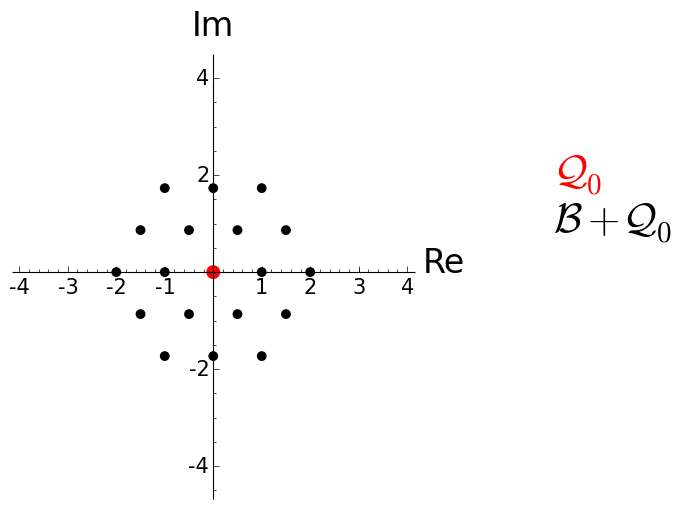
\includegraphics[height=0.8\textheight]{img/eisenstein/phase1_image_2} \hfill
            \vfill
          } 
\only<2>{%
            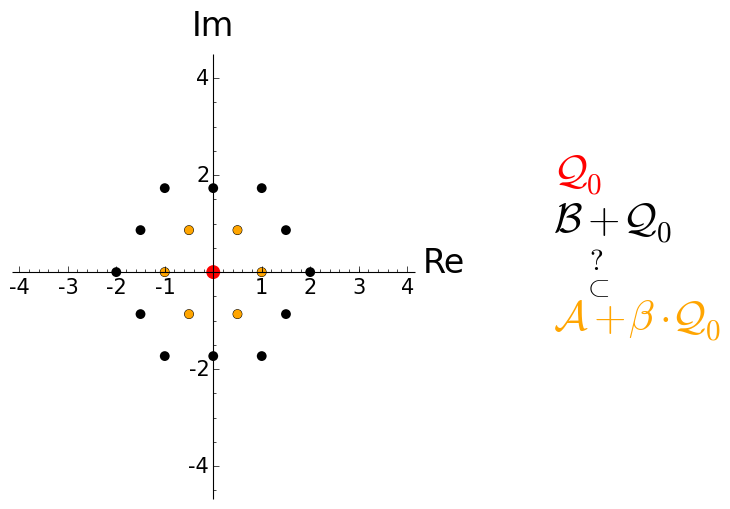
\includegraphics[height=0.8\textheight]{img/eisenstein/phase1_image_3} \hfill
            \vfill
          }                     

\only<3>{%
            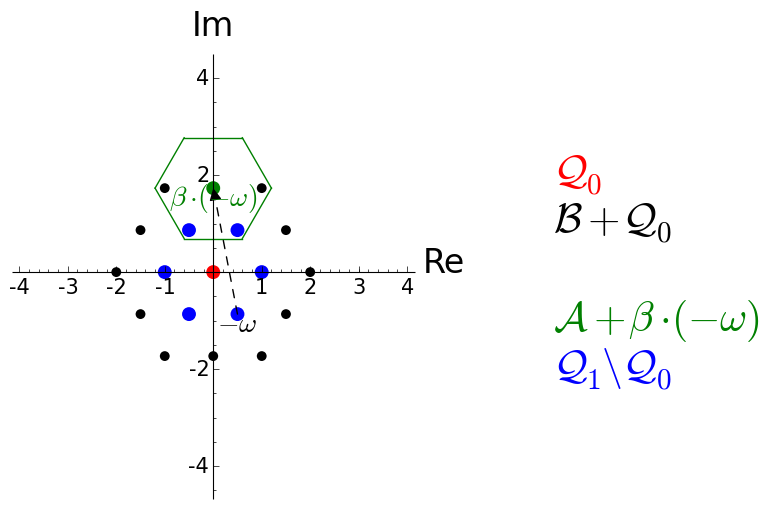
\includegraphics[height=0.8\textheight]{img/eisenstein/phase1_image_4} \hfill
            \vfill
          } 
\only<4>{%
            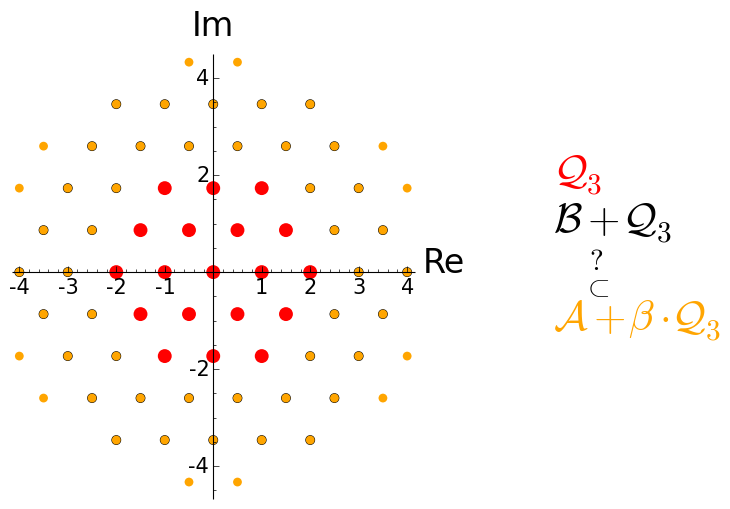
\includegraphics[height=0.8\textheight]{img/eisenstein/phase1_image_12} \hfill
            \vfill
          }
\only<5>{%
            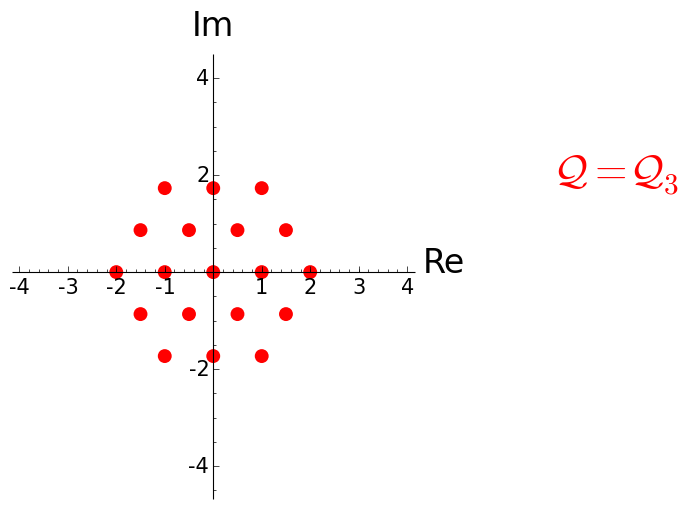
\includegraphics[height=0.8\textheight]{img/eisenstein/phase1_image_13} \hfill
            \vfill
          }
\end{frame}

\subsection{Fáze 2 -- váhová funkce}
\begin{frame}
    \frametitle{Fáze 2 -- hledání váhové funkce}

    Hledáme šířku okna $M$ a váhovou funkci $q:(\A+\A)^{M} \to \Q$ takovou, že
    $$
    z_j=w_j + \underbrace{q(w_{j-1}, \dots, w_{j-M})}_{=q_{j-1}} - \underbrace{q(w_j, \dots, w_{j-(M-1)})}_{=q_{j}} \beta \in \A \,.
    $$
    
%    Pro šířku okna $m$ určíme $q_j\in\Q_{[w_{j},\dots, w_{j-m+1}]}\subset \Q$
%    
%    Zkontrolujeme všechny přenosy zprava $q_{j-1}$ a určíme $q_j\in\Q$ takové, že 
%    $$
%    z_j=w_j + q_{j-1} - q_j \beta \in \A \,.
%    $$
%        
%    \pause
%    Šířka okna $M$ a váhová funkce $q$ je nalezena, když 
%    $$
%    \#\Q_{[w_{j},\dots, w_{j-M+1}]}=1
%    $$
%    pro všechny  $w_{j},\dots, w_{j-M+1} \in (\A+\A)^M$.
\end{frame}    




% \begin{frame}
%     \frametitle{Příklad -- fáze 2}
%     Předpokládejme vstup  $(\omega\, 1\, 2)$.
% \end{frame}

\begin{frame}
\only<1-2>{Vstup: $(\omega)$}
\only<3>{Vstup: $(\omega\, 1)$}
\only<4>{Vstup: $(\omega\, 1\, 2)$}

\only<1>{%
        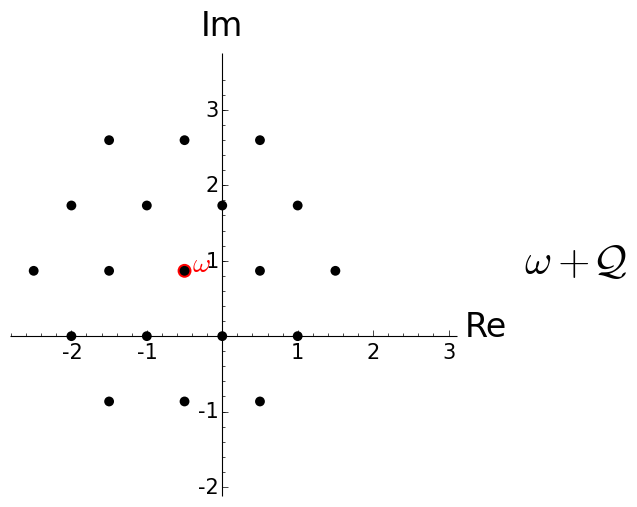
\includegraphics[height=0.7\textheight]{img/eisenstein/phase2_image_2} \hfill
        \vfill
          }  
\only<2>{%
        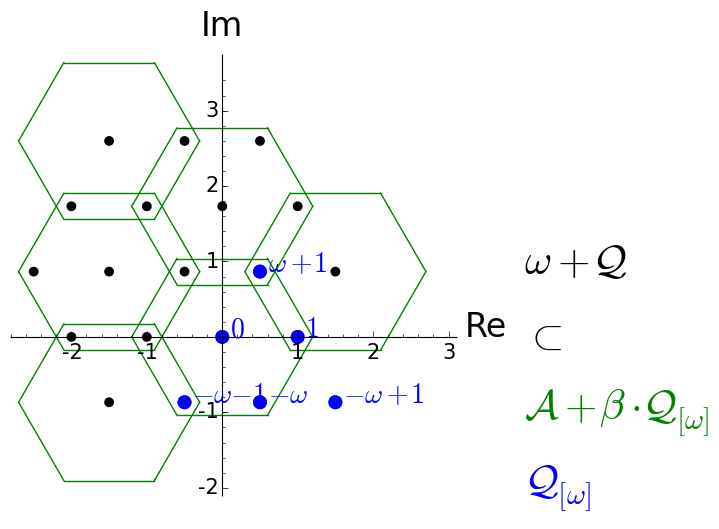
\includegraphics[height=0.7\textheight]{img/eisenstein/phase2_image_3} \hfill
        \vfill
          }  
\only<3>{%
        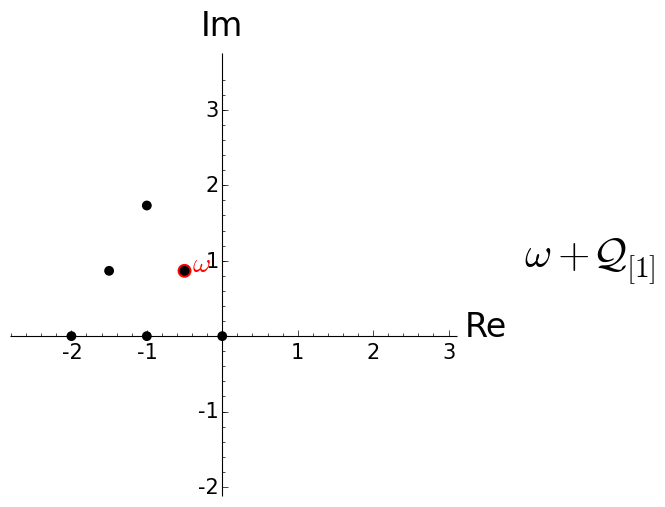
\includegraphics[height=0.7\textheight]{img/eisenstein/phase2_image_4} \hfill
        \vfill
          }  
\only<4>{%
        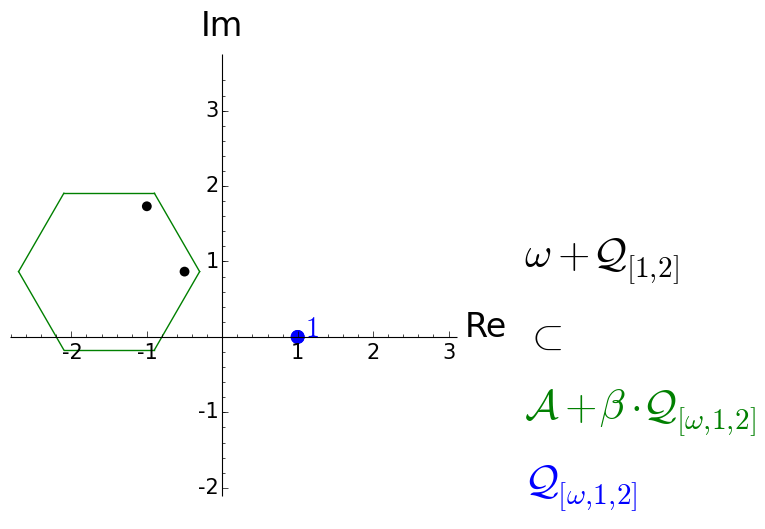
\includegraphics[height=0.7\textheight]{img/eisenstein/phase2_image_7} \hfill
        \vfill
          }           
\end{frame}

\section{Konvergence}
\subsection{Abeceda}
\begin{frame}
    \frametitle{Dolní odhad velikosti abecedy}
Abeceda $\A\subset \Zbeta$ taková, že $0\in \A$ a $1\in \A[\beta]$.

Pokud existuje algoritmus pro paralelní sčítání v poziční soustavě $(\beta, \A)$, který používá přepisovací pravidlo $x-\beta$, pak
$$
\#\A \geq \max \{|m_\beta(0)|, |m_\beta(1)|\}\,,
$$
kde $m_\beta$ je minimální polynom báze $\beta$.
Navíc, pokud $\beta$ má reálný sdružený kořen větší než 1, pak
$$
\#\A \geq \max \{|m_\beta(0)|, |m_\beta(1)|+2\}\,.
$$
\end{frame}

\subsection{Fáze 1}
\begin{frame}
\frametitle{Fáze 1 -- postačující a nutná podmínka konvergence}
Nechť abeceda $\A\subset\Zomega$ obsahuje alespoň jednoho reprezentanta každé třídy kongruence modulo $\beta$ v $\Zomega$. 

\vspace{1cm}
Pokud je $\beta$ expandující, pak Fáze 1 konverguje.

\vspace{1cm}
Naopak, pokud existuje algoritmus pro paralelní sčítání v soustavě $(\beta,\A)$ s přepisovacím pravidlem $x-\beta$, pak je $\beta$ expandující.


\end{frame}

\subsection{Fáze 2}
\begin{frame}
\frametitle{Fáze 2 -- zastavovací podmínka}
%Vrcholy Rauzyho grafu Fáze 2 pro šířku okna $k$ jsou kombinace $(w_{-1}, \dots ,w_{-k})\in(\A+\A)^k$ takové, že 
%$$\#\Q_{[w_{-1},\dots, w_{-k}]}=\#\Q_{[w_{-1},\dots, w_{-(k-1)}]}\,.$$
%
%\vspace{1cm}
%Z $(w_{-1}, \dots ,w_{-k})$ do $(w'_{-1}, \dots ,w'_{-k})$ vede hrana právě tehdy, když
%\begin{align*}
% (w_{-2}, \dots,w_{-k})=(w'_{-1}, \dots, w'_{-(k-1)})\,.
%\end{align*}

Nechť $w_0,w_{-1},\dots, w_{-k}\in(\A+\A)$ jsou takové, že $\#\Q_{[w_{0},\dots, w_{-k}]}=\#\Q_{[w_{0},\dots, w_{-(k-1)}]}>1$. 

\vspace{1cm}
Pokud existuje nekonečná cesta v tzv. Rauzyho grafu Fáze 2 pro šířku okna $k$ začínající hranou $(w_{0}, \dots ,w_{-(k-1)})\rightarrow (w_{-1}, \dots ,w_{-k})$, pak ve Fázi 2 došlo k zacyklení.
\end{frame}


\section{Výsledky}
\begin{frame}
\fontsize{8pt}{10}\selectfont
    \frametitle{Testované příklady}
    \begin{tabular}{c|cc| cc c| c| c c }
$\omega$ & $\beta$ & $m_\beta$  & $\#\A$ & $\A\subset$ & min. & $\#\Q$ &  Ph. 2 & $M$   \\ \hline
 $ \frac{1}{2} i \, \sqrt{11} - \frac{1}{2} $ & $ i \, \sqrt{11} - 4 $ & $ x^{2} + 8 \, x + 27 $  & $ 36 $ & $\Zomega$ & yes & $ 13 $ & \checkmark & 5 \\
 $ \frac{1}{2} i \, \sqrt{7} - \frac{1}{2} $ & $ \frac{1}{2} i \, \sqrt{7} - \frac{1}{2} $ & $ x^{2} + x + 2 $ & $ 4 $ & $\Zomega$ & yes & $ 29 $ & \checkmark & 8 \\
 $ \frac{1}{2} i \, \sqrt{3} + \frac{1}{2} $ & $ -i \, \sqrt{3} - 1 $ & $ x^{2} + 2 \, x + 4 $  & $ 8 $ &  $\Zomega$ & no & $ 23 $ & \checkmark & 5 \\
 $ i $ & $ -3 i - 3 $ & $ x^{2} + 6 \, x + 18 $  & $ 25 $ & $\Zomega$ & yes & $ 15 $ & \checkmark & 4 \\
 $ -\frac{1}{2} \, \sqrt{5} + \frac{3}{2} $ & $ \frac{3}{2} \, \sqrt{5} - \frac{15}{2} $ & $ x^{2} + 15 \, x + 45 $  & $ 61 $ & $\Zomega$ & yes & $ 15 $ & \checkmark & 3 \\
 $ -\frac{1}{2} \, \sqrt{5} + \frac{3}{2} $ & $ \sqrt{5} - 5 $ & $ x^{2} + 10 \, x + 20 $  & $ 31 $ & $\Zomega$ & yes & $ 11 $ & \checkmark & 3 \\
 $ \frac{1}{2} \, \sqrt{17} - \frac{3}{2} $ & $ \frac{1}{2} \, \sqrt{17} - \frac{9}{2} $ & $ x^{2} + 9 \, x + 16 $  & $ 26 $ & $\Zomega$ & yes & $ 17 $ & \checkmark & 5 \\
$ \frac{1}{2} i \, \sqrt{11} + \frac{1}{2} $ & $ -i \, \sqrt{11} $ & $ x^{2} + 11 $  & $ 13 $ & $\ZZ$ & no & $ 9 $ & \checkmark & 2 \\
$ \frac{1}{2} i \, \sqrt{11} + \frac{1}{2} $ & $ -i \, \sqrt{11} $ & $ x^{2} + 11 $  & $ 12 $ & $\ZZ$ & yes & $ 9 $ & \checkmark & 4 \\
$ \frac{1}{2} i \, \sqrt{7} - \frac{1}{2} $ & $ -i \, \sqrt{7} $ & $ x^{2} + 7 $  & $ 8 $ & $\ZZ$ & yes & $ 9 $ & \checkmark & 4   \\
$ \frac{1}{2} i \, \sqrt{3} + \frac{1}{2} $ & $\! -\frac{3}{2} i \sqrt{3} + \frac{1}{2}\!$ & $\! x^{2} - x + 7 \!\!$ & $ 11 $ & $\ZZ$ & no & $ 9 $ & \checkmark & 2  \\
$ \sqrt{6} - 1 $ & $ \sqrt{6} $ & $ x^{2} - 6 $  & $ 7 $ & $\ZZ$ & yes & $ 9 $ & \checkmark & 4 \\
$ -\sqrt{7} + 2 $ & $ \sqrt{7} $ & $ x^{2} - 7 $  & $ 8 $ & $\ZZ$ & yes & $ 9 $ & \checkmark & 4 \\
$ -\frac{1}{2} \, \sqrt{21} + \frac{3}{2} $ & $ -\sqrt{21} $ & $ x^{2} - 21 $  & $ 22 $ & $\ZZ$ & yes & $ 9 $ & \checkmark & 4 \\
$ \sqrt[3]{2} $ & $ -\sqrt[3]{2} $ & $ x^{3} + 2 $ & $ 3 $& $\ZZ$  & yes & $ 27 $ &  \checkmark & 6 \\
$ \sqrt[3]{2} $ & $ \sqrt[3]{2} $ & $ x^{3} - 2 $ & $ 3 $ & $\ZZ$ & yes & $ 27 $ &  \checkmark & 6 \\
\end{tabular}

\end{frame}

\begin{frame}
    \frametitle{Výsledky}    
	Konvergence:
    \begin{itemize}
        \item dolní odhad velikosti abecedy ze $\Zbeta$
        \item nutná a postačující podmínka konvergence Fáze 1
        \item algoritmus pro odhalování zacyklení fáze 2
    \end{itemize}
    \pause
    Implementace v SageMath:
    \begin{itemize}
        \item extending window method včetně mnoha různých možností výběru v obou fázích
        \item navržený algoritmus pro odhalování zacyklení fáze 2
        \item generování možné abecedy k zadané bázi
    \end{itemize}    
    \pause
    Testování
    \begin{itemize}
	    \item velké množství vstupů (díky automatickému ukládání do google tabulky)
	    \item úspěšné nalezení algoritmu paralelního sčítání pro téměř 140 pozičních soustav
    \end{itemize}
\end{frame}


\begin{frame}
\fontsize{14pt}{10}\selectfont
\begin{center}
Děkuji

\end{center}    

\end{frame}
%
%
%\begin{frame}
%    Množinu $\Q$ konstruujeme iterativně:
%    \begin{block}{Fáze 1}
%     $k:=0$
%     
%    $\Q_0:=\{0\}$
%      
%      \pause
%      Repeat:
%      \begin{itemize}
%          \item rozšiř $\Q_k$ na $\textcolor{red}{\Q_{k+1}}$ tak, že
%           $$
%              (\A+\A)+ \Q_k \subset \A + \beta \textcolor{red}{\Q_{k+1}}\,,
%           $$
%           \item $k:=k+1$
%      \end{itemize}
%      \pause
%      until $\Q_k = \Q_{k+1}$.
%      
%      \pause
%      \vspace{7pt}
%      $\Q:=\Q_k$
%    \end{block}
%\end{frame}
%
%
%
%\begin{frame}
%    \begin{block}{Fáze 2}
%      $m:=1$
%      
%      Pro každé $w_j \in \A+\A$ najdi množinu $\Q_{[w_j]} \subset \Q$ takovou, že
%      $$
%      w_j + \Q \subset \A + \beta \Q_{[w_j]}
%      $$
%    \pause
%      While $(\max\{\#\Q_{[w_j,\dots, w_{j-m+1}]}:(w_j,\dots, w_{j-m+1}) \in (\A+\A)^m \} > 1)$ do:
%      \begin{itemize}
%          \pause
%          \item $m:= m +1$
%          \pause
%          \item Pro všechny $(w_j,\dots, w_{j-m+1}) \in (\A+\A)^{m}$ najdi množinu $\textcolor{red}{\Q_{[w_j,\dots, w_{j-m+1}]}} \subset \Q_{[w_j,\dots, w_{j-m+2}]}$ takovou, že
%          $$
%          w_j + \Q_{[w_{j-1},\dots, w_{j-m+1}]} \subset \A + \beta \textcolor{red}{\Q_{[w_j,\dots, w_{j-m+1}]}}\,,
%          $$
%      \end{itemize}
%      \pause
%      $M:= m$ 
%      
%      \pause
%      $q(w_j,\dots, w_{j-M+1}):=$ jediný prvek $\Q_{[w_j,\dots, w_{j-M+1}]}$
%    \end{block}
%\end{frame}

\end {document}


